\documentclass{article}
\usepackage{graphicx} % Required for inserting images
\usepackage{float}
\usepackage{caption}


\title{Parallel and Distributed Computing - First Project Report - FEUP 24/25 - 2nd Semester} 

\author{
Turma 07 Grupo 11 \\
Carlos Sanches, up202107694 \\
João Rebelo, up202107209 \\
Luís Ganço, up202004196
}
\date{March 21, 2025}

\begin{document}

\newpage 

\maketitle
\begin{center}
    \large \textit{Project Theme:} Performance Comparison of Single-Core and Multi-Core Systems
\end{center}
\newpage
% Add the table of contents (index)
\tableofcontents
\newpage % Start a new page after the table of contents

\section{Introduction}

\subsection{Problem Description}
In modern computing, the performance of processors is heavily influenced by the memory hierarchy, particularly when handling large datasets. Matrix multiplication, a fundamental operation in many scientific and engineering applications, serves as case study to explore these performance dynamics. This project aims to evaluate the impact of memory hierarchy on processor performance by implementing and analyzing different versions of matrix multiplication algorithms in multiple programming languages.

The project is divided into two main parts: single-core and multi-core performance evaluations. In the single-core evaluation, we implement and compare matrix multiplication algorithms in C/C++ with Java. We measure processing times for matrices of varying sizes and analyze the effects of different algorithmic approaches, including a block-oriented implementation. The Performance API (PAPI) is utilized to collect relevant performance metrics, such as cache misses and floating-point operations, to provide deeper insights into the behavior of the memory hierarchy.

For the multi-core evaluation, we parallelize the matrix multiplication algorithms using OpenMP and analyze their performance in terms of MFlops, speedup, and efficiency. Two parallelization strategies are explored, and their results are compared to understand the trade-offs between different parallel implementations.

This report documents the implementation details, performance metrics, and analysis of the results obtained from both single-core and multi-core evaluations. 

\subsection{Algorithms Explanation}

\subsubsection{Matrix Multiplication Algorithm}

\begin{itemize}
    \item Element-wise multiplication and summation: each element of a row is multiplied by the corresponding element of a column, and all of them are summed up;
    \item Time complexity: O(n³), the algorithm has three nested for loops.
\end{itemize}

\section{Performance Metrics}

We decided to use the following metrics to evaluate performance:

\begin{itemize}
    \item \textbf{Execution Time - } Measures the total time taken to complete matrix multiplication for different matrix sizes. This metric provides a straightforward way to compare the overall efficiency of the implementations in C++ and Java.
    
    \item \textbf{Data Cache Misses (DCM) - } Tracks the number of times data requested by the CPU is not found in the cache, requiring slower memory access. We analyzed both L1 and L2 cache misses to better understand how memory access patterns impact performance, especially for larger matrix sizes.
    
    \item \textbf{FLOPS (MFlops and GFlops) - } Measures the number of floating-point operations per second, reflecting the raw computational throughput. In accordance with the assignment requirements, we used MFlops for the second part of the work. However, we also included GFlops to provide a more complete performance evaluation, as it better captures the scale of larger matrices.
\end{itemize}

This combination of metrics allowed us to assess not only how fast the algorithms run but also how efficiently they utilize the hardware, considering both computation and memory access patterns.

\section{Results and Analysis}

\subsection{Multiplication}

\begin{table}[H]
\centering
\caption{C++ Performance Results}
\begin{tabular}{||c | c | c | c | c||} 
 \hline
 \textbf{Dimensions} & \textbf{Execution Time (s)} & \textbf{GFlops} & \textbf{L1 DCM} & \textbf{L2 DCM} \\  
 \hline \hline
 600x600  & 0.154   & 2.80   & 241678983   & 448582    \\  
 \hline
 1000x1000 & 0.702   & 2.85   & 1136969844 & 3488117  \\  
 \hline
 1400x1400 & 2.846   & 1.93   & 3125017136 & 58169452 \\  
 \hline
 1800x1800 & 6.711   & 1.74   & 7059740261 & 94416650 \\  
 \hline
 2200x2200 & 16.870  & 1.26   & 15939144633 & 558295715 \\  
 \hline
 2600x2600 & 41.912  & 0.84   & 30910168160 & 2305966036 \\  
 \hline
 3000x3000 & 67.189  & 0.80   & 50421145206 & 6043903995 \\  
 \hline
\end{tabular}
\end{table}

\begin{table}[H]
\centering
\caption{Java Performance Results}
\begin{tabular}{||c | c | c||} 
 \hline
 \textbf{Dimensions} & \textbf{Execution Time (s)} & \textbf{GFlops} \\  
 \hline \hline
 600x600  & 0.254   & 1.70   \\  
 \hline
 1000x1000 & 1.581   & 1.27   \\  
 \hline
 1400x1400 & 8.502   & 0.65   \\  
 \hline
 1800x1800 & 23.912  & 0.49   \\  
 \hline
 2200x2200 & 51.042  & 0.42   \\  
 \hline
 2600x2600 & 104.170 & 0.34   \\  
 \hline
 3000x3000 & 175.885 & 0.31   \\  
 \hline
\end{tabular}
\end{table}

After comparing the performance results of C++ and Java, it is clear that C++ is faster. To confirm this, we plotted relevant graphs comparing the performance metrics of both languages, as shown below:

\begin{figure}[H]
    \centering
    \begin{minipage}{0.32\textwidth}
        \centering
        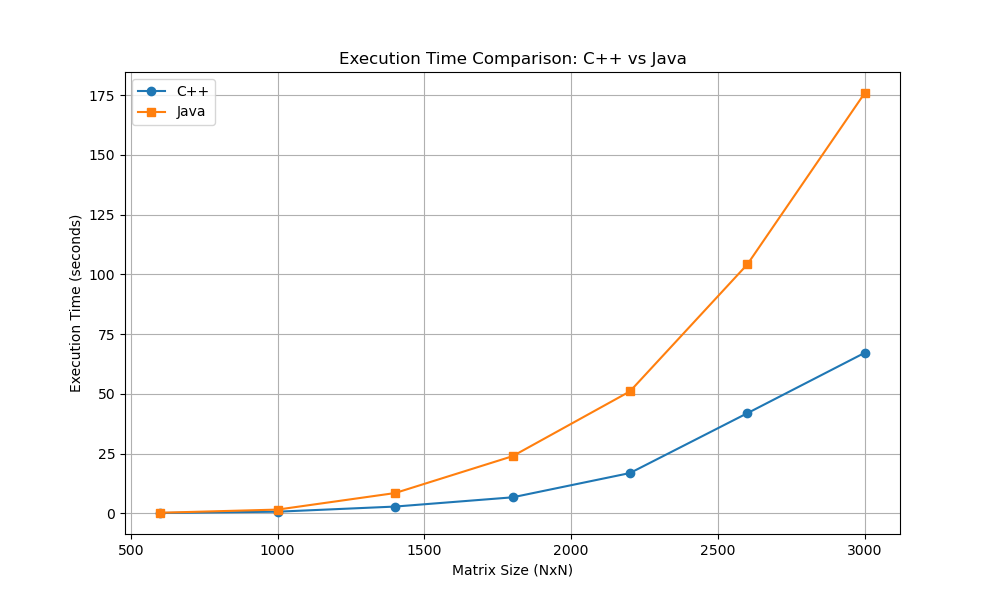
\includegraphics[width=\textwidth]{Figure_1.png}
        \caption{\small Execution Time Comparison}
        \label{fig:execution_time}
    \end{minipage}
    \hfill
    \begin{minipage}{0.32\textwidth}
        \centering
        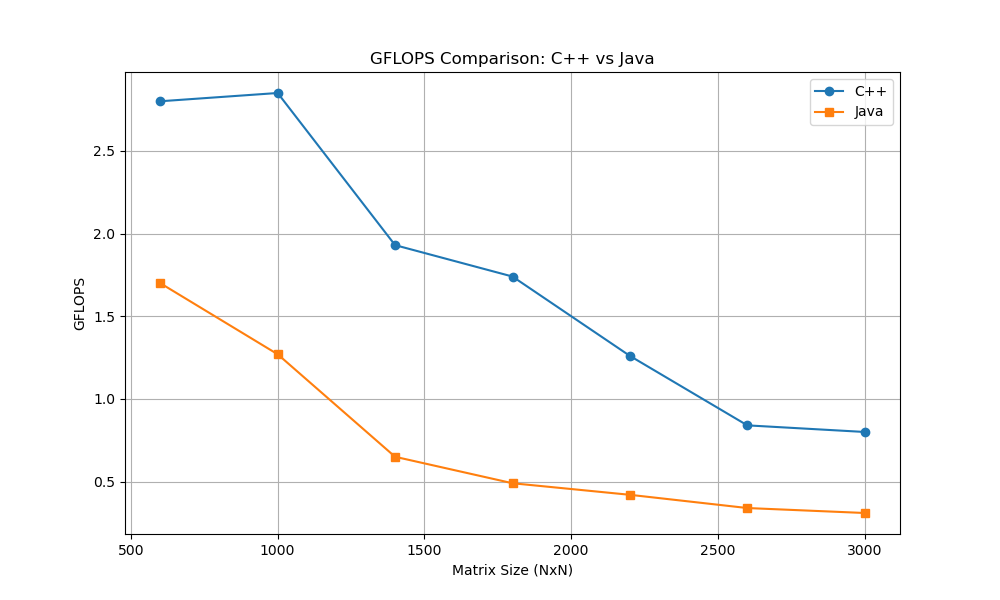
\includegraphics[width=\textwidth]{Figure_2.png}
        \caption{\small GFlops comparison}
        \label{fig:flops}
    \end{minipage}
    \hfill
    \begin{minipage}{0.32\textwidth}
        \centering
        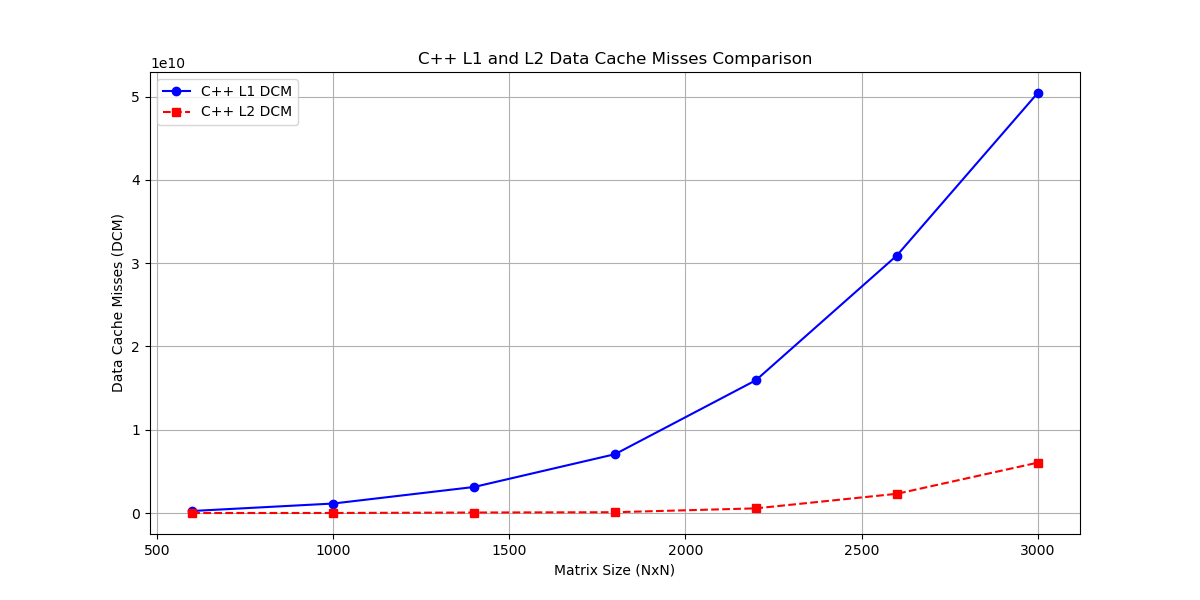
\includegraphics[width=\textwidth]{Figure_3.png}
        \caption{\small C++ DCM Comparison}
        \label{fig:cache_misses}
    \end{minipage}
\end{figure}

Figure 1 supports our initial observation, while Figures 2 and 3 provide valuable insights into the underlying factors affecting performance:

\begin{itemize}
    \item C++ outperforms Java consistently across all matrix sizes, with higher GFlops values;
    \item As the matrix size grows, performance (GFlops) decreases for both languages, but the drop is sharper for Java;
    \item This shows that C++ handles large matrix multiplications more efficiently, likely due to better memory management and lower runtime overhead;
    \item L1 cache misses grow exponentially as matrix size increases, indicating that larger matrices don't fit well in the smaller, faster L1 cache;
    \item L2 cache misses are much lower, but they still increase gradually, highlighting that more data spills into higher cache levels;
    \item This pattern suggests that performance degradation for larger matrices is tied to cache inefficiencies, with more memory accesses going to slower cache layers or RAM.
\end{itemize}


\section{Conclusions}

\end{document}
